\documentclass{homework}

\linespread{1.2}

\usepackage[T1]{fontenc}\usepackage{palatino}
\usepackage{amssymb,amsmath,amsthm,mathtools}
\usepackage[english]{babel}
\usepackage[utf8]{inputenc}
\usepackage[babel]{csquotes}
\usepackage[pdftex]{hyperref}
\usepackage{enumitem}
\usepackage[usenames,dvipsnames,table,xcdraw]{xcolor}

\usepackage{graphicx} 
\usepackage{verbatim} % Commenti in blocco con \begin{comment}
\usepackage{bm}
\usepackage[font={small,it}]{caption}
\usepackage{subcaption}
\usepackage{geometry}
\usepackage{array}
\usepackage{enumitem}
\setlist[enumerate]{label*=\arabic*.}
	
\usepackage{algorithm}
\usepackage[noend]{algpseudocode}
\usepackage{listings}

\definecolor{mygraybackground}{gray}{0.95}

% Define the R listings to write code
\lstset{
  language=R,
  basicstyle=\scriptsize\ttfamily, 
  numbers=left,
  numberstyle=\small\ttfamily\color{Gray},
  numbersep=10pt,
  backgroundcolor=\color{mygraybackground},
  showstringspaces=false,
  showtabs=false,
  tabsize=3,
  breaklines=true,
  captionpos=b,   
  keywordstyle=\color{black},
  commentstyle=\color{ForestGreen},
}

\makeatletter
\def\BState{\State\hskip-\ALG@thistlm}
\makeatother

% Simbolo iid
\newcommand\iid{\stackrel{\mathclap{\normalfont\tiny\mbox{iid}}}{\sim}}
% Simbolo ind
\newcommand\ind{\stackrel{\mathclap{\normalfont\tiny\mbox{ind}}}{\sim}}

\title{SDS 385: Homework 2}
\author{G.~Paulon}

\begin{document}

\makeatletter
\begin{titlepage}
	\vspace*{\fill}
	\centering
	{\huge \@title \par}
	\vskip0.5cm
	{\large \@author \par}
	\vskip0.5cm
	{\large \today \par}
	\vspace*{\fill}
\end{titlepage}
\makeatother

\newpage 
\mbox{}
\thispagestyle{empty}
\newpage

\setcounter{page}{1}

\problem{SGD for logistic regression}

\begin{enumerate}[label=(\Alph*)]

\item In part (A) of the last homework we proved that the gradient of the negative log-likelihood can be expressed as
\begin{equation*}
\nabla l(\beta) = - \sum_{i=1}^n \left\lbrace x_i (y_i - m_i w_i) \right\rbrace = \sum_{i=1}^n g_i (\beta)
\end{equation*}
where
\begin{equation*}
g_i (\beta) = x_i (y_i - m_i w_i) = x_i (y_i - \hat{y}_i)
\end{equation*}
and
\begin{equation*}
\hat{y}_i = \mathbb{E} (y_i | \beta) = m_i w_i (\beta) = m_i \frac{1}{1+\exp(-x_i^T \beta)}.
\end{equation*}
A nice interpretation can be given to this latter expression: the gradient is large when the data $y_i$'s differ from their maximum likelihood estimates, i.e. the probabilities $w_i$'s.

\item

\item The SGD exploits this fact in order to use an update step which is faster to compute. In fact, instead of using the gradient calculated from all $n$ data points to choose the step direction, we use the gradient $g_i(\beta)$ calculated from a single data point, sampled randomly from the whole data set. In this version of the algorithm, sampling without replacement has been performed. 

In order to asses the validity of the implementation, we run the algorithm on the real data for a reasonable number of iterations $N = 100000$. We tried different values for the step size $\gamma$, which was kept constant over the iterations. We report in Figures \ref{fig:a001} - \ref{fig:a1} the traceplots of all of the $\beta$ parameters (i.e. the values of the parameters over the iterations). In order to facilitate the visualization, we thinned the samples by a factor $20$ (we displayed one value of $\beta$ every $20$ iterations). 

We can see that for small values of the step size $\gamma$, convergence is not reached for many of the components of $\beta$. When we increase the step size, on the other hand, convergence is reached more rapidly because the algorithm explores well the parameters space. However, the asymptotic variance of the parameters is higher, since at every iteration the weight attributed to the direction given by any new sampled data is high. 

In this first implementation of the algorithm we do not worry about the choice of the tuning parameter, that is instead crucial for SGD. As a convergence diagnostics, we plot the iterates of the running average of $l_t(\beta)$, the individual log-likelihood contribution from the data point sampled at step $t$.

\begin{figure}[!ht]
\centering
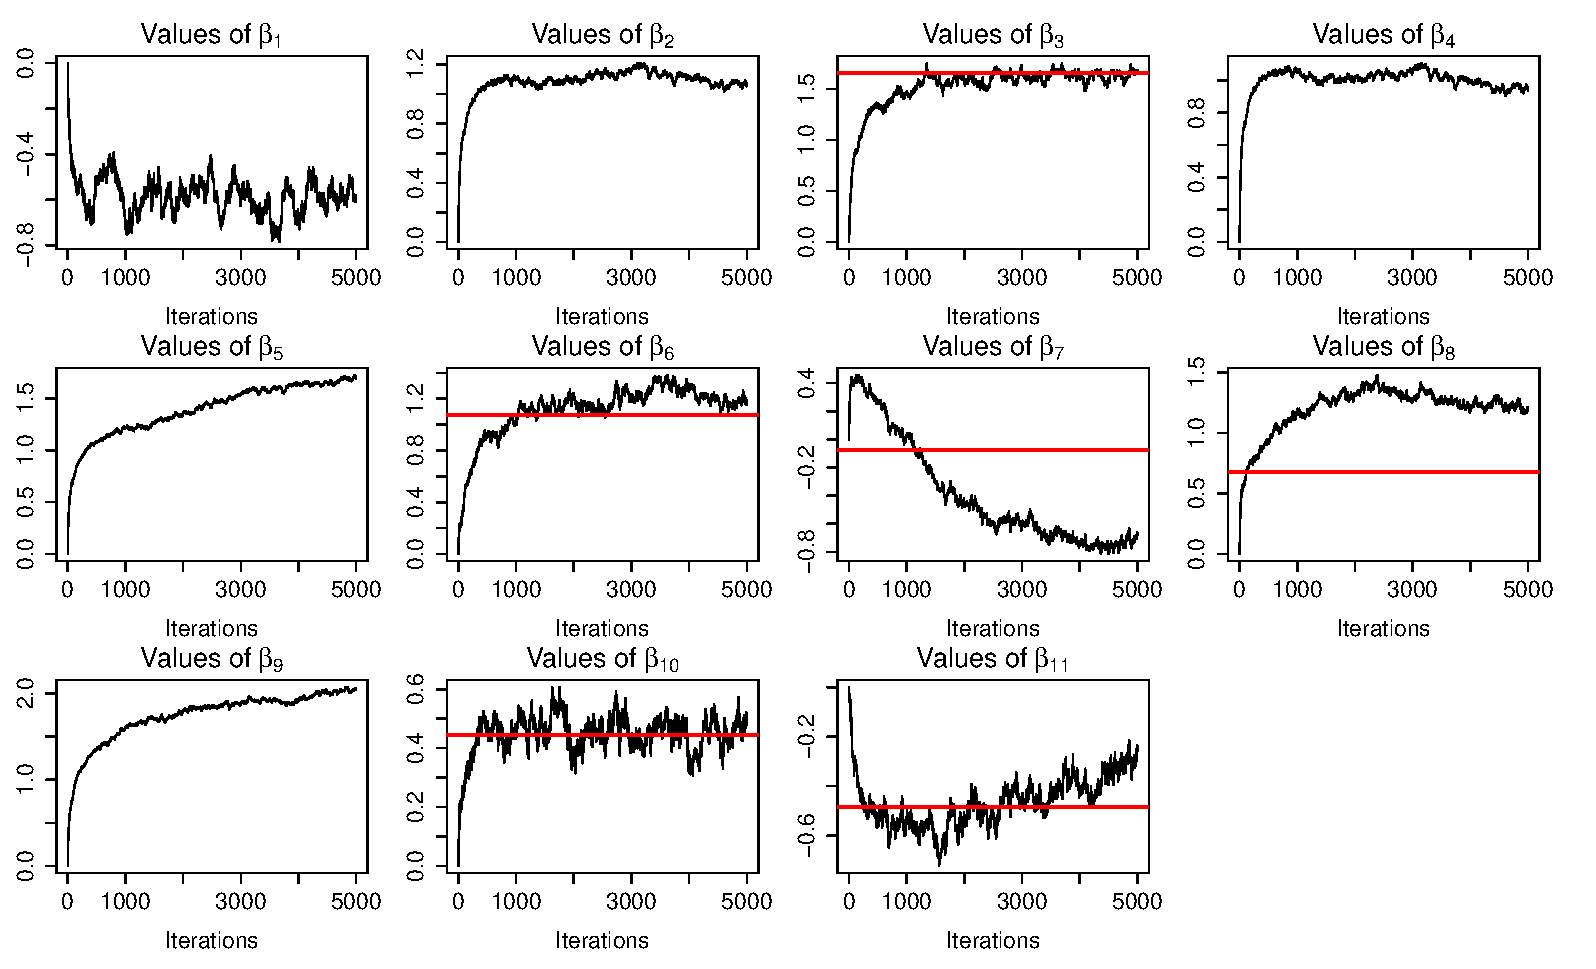
\includegraphics[width=0.9\columnwidth]{./Img/a001}
\caption{Traceplots of the $\beta$ parameters when $\gamma = 0.01.$}
\label{fig:a001}
\end{figure}

\begin{figure}[!ht]
\centering
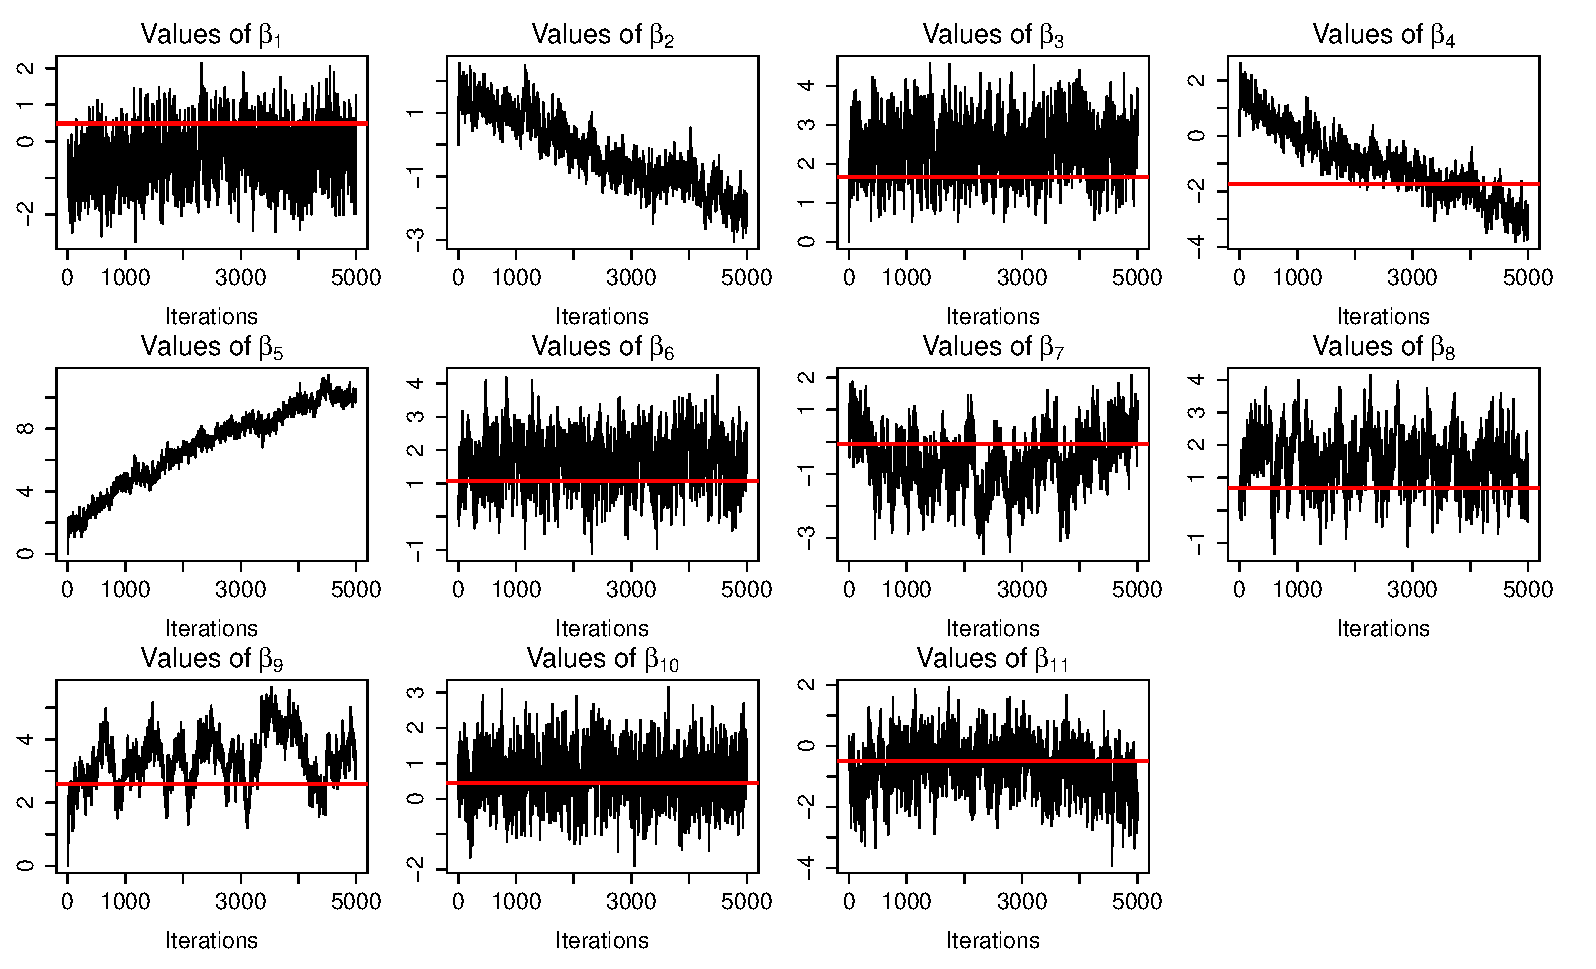
\includegraphics[width=0.9\columnwidth]{./Img/a05}
\caption{Traceplots of the $\beta$ parameters when $\gamma = 0.5.$}
\label{fig:a05}
\end{figure}

\begin{figure}[!ht]
\centering
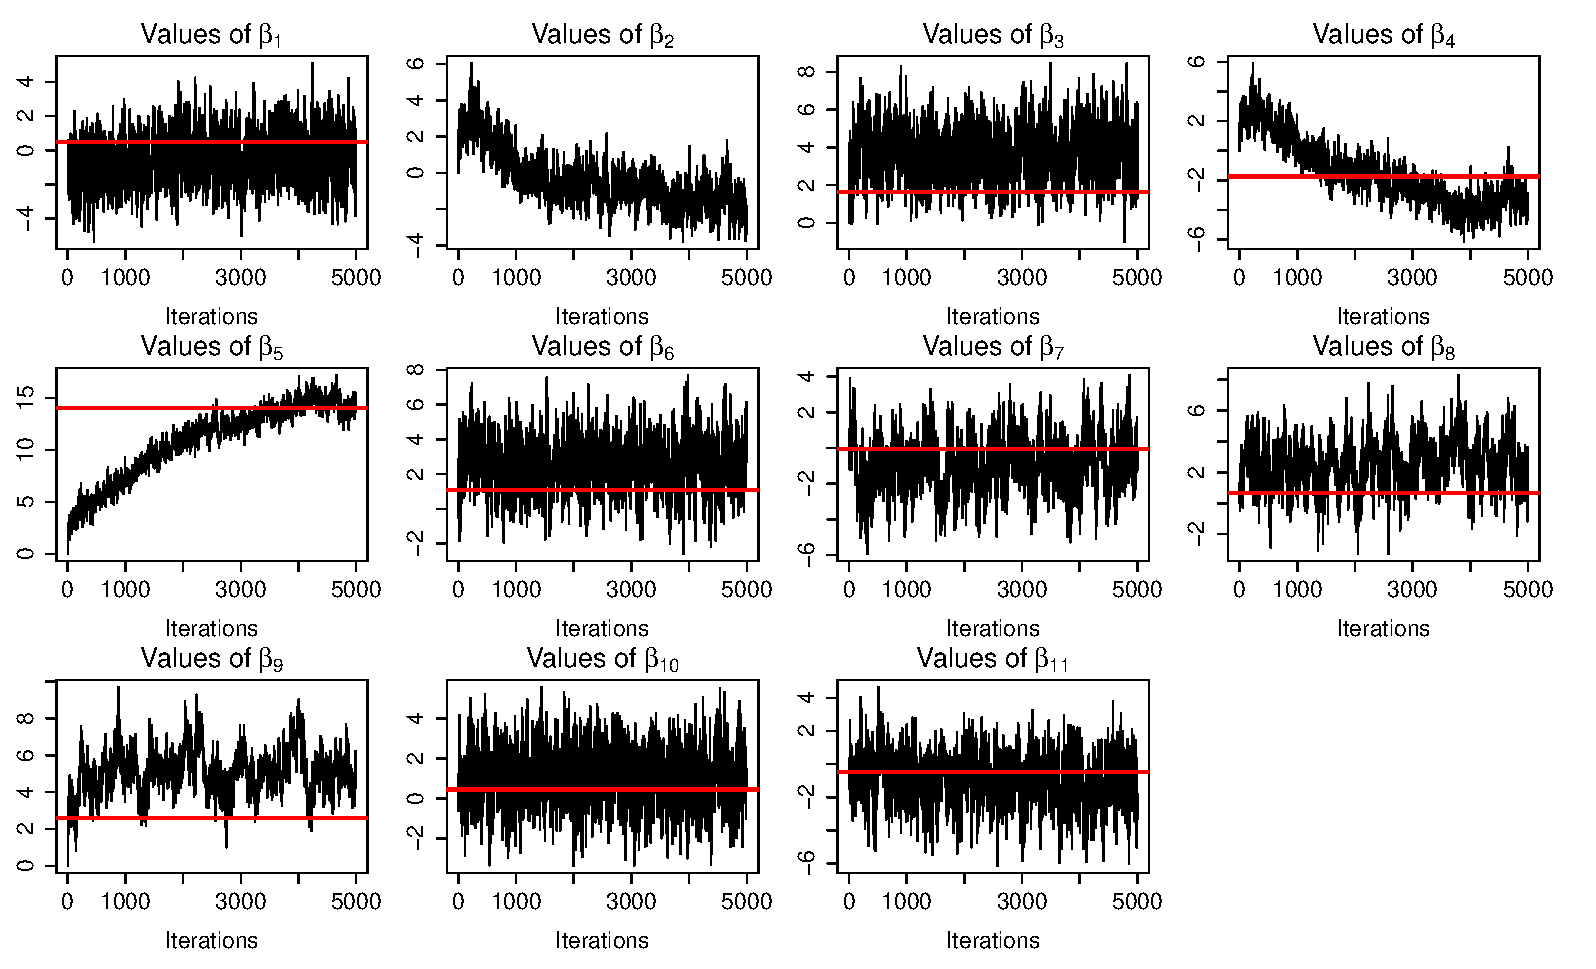
\includegraphics[width=0.9\columnwidth]{./Img/a1}
\caption{Traceplots of the $\beta$ parameters when $\gamma = 1.$}
\label{fig:a1}
\end{figure}

\begin{figure}[!ht]
\centering
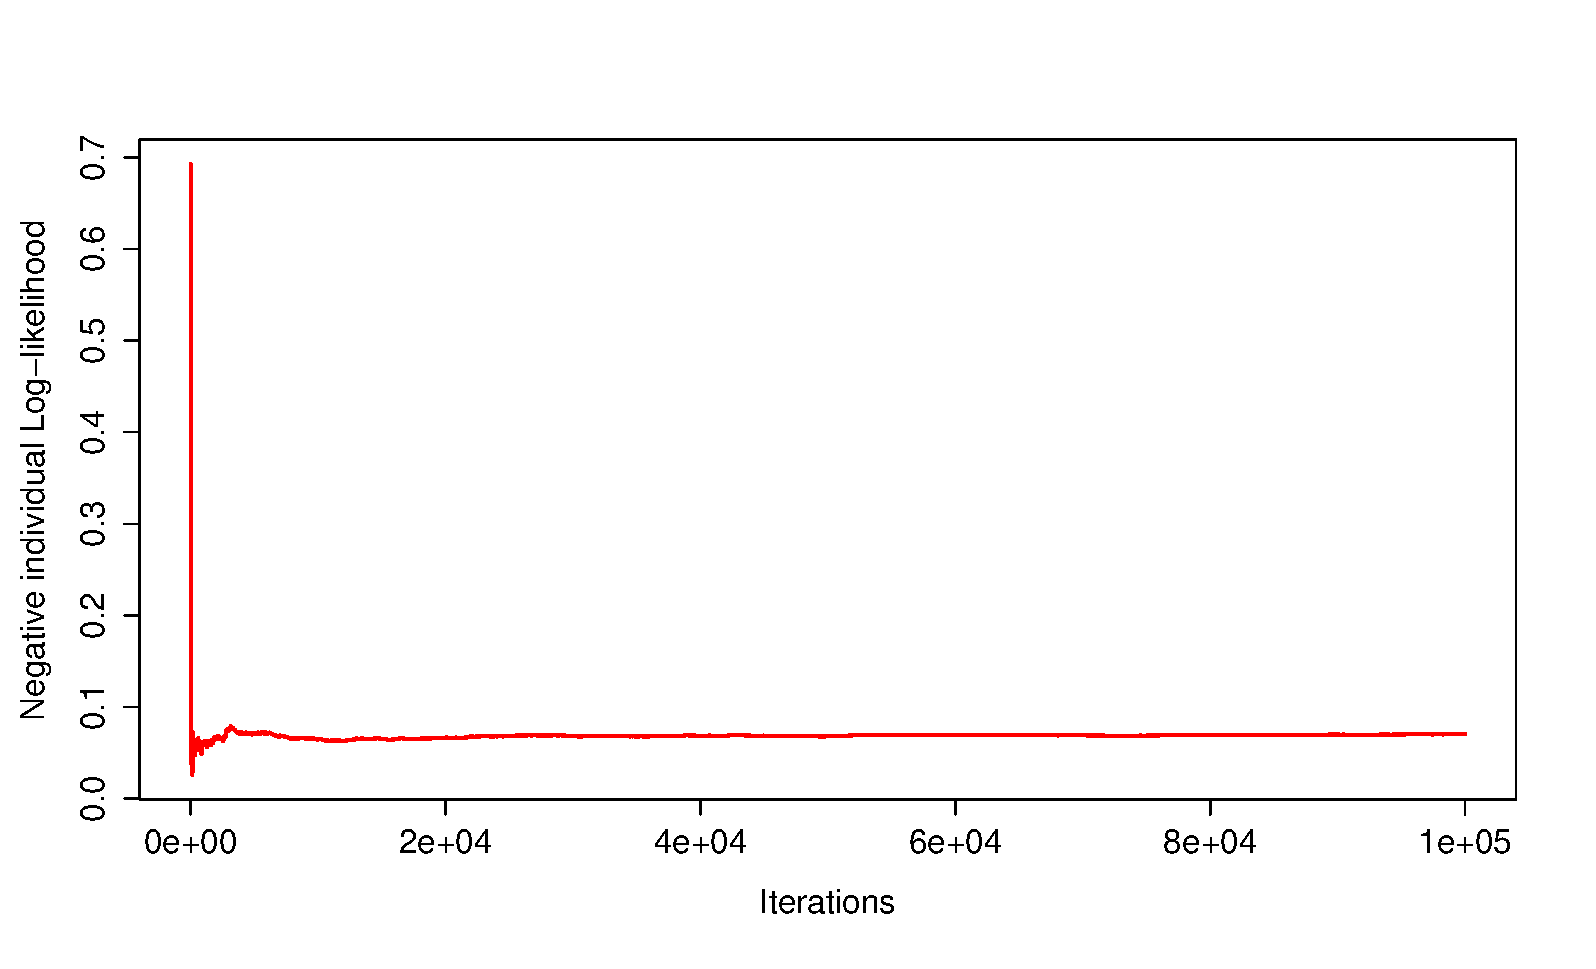
\includegraphics[width=0.9\columnwidth]{./Img/ll}
\caption{Running average of the single log-likelihood contributions.}
\label{fig:loglikelihood}
\end{figure}

\clearpage

\item Now we try using a decaying step size. Specifically, we use the Robbins–Monro rule for step sizes:
$$\gamma(t) = C(t+t_0)-\alpha,$$
where $C > 0$, $\alpha \in [0.5, 1]$, and $t_0$ (the ``prior number of steps'') are constants. The exponent $\alpha$ is usually called the learning rate. 

Ideally, we want to obtain large values of $\gamma$ at the beginning of the algorithms, so that the ``true'' values of the parameters are rapidly reached. Afterwards, we want the step sizes to be reduced in order to diminish the variance of the estimates and to, eventually, converge.

\item

\end{enumerate}


\end{document}
